\section{ロボカー}
\subsection{機体}
\refig{figure1}に配布されたロボカーのベース部を示す.本体の前方には前輪を駆動させロボカーを旋回させるためのサーボモータを設置した.そして,ロボカーの後方には後輪を駆動させ機体を動かすためのDCモータと角速度を計測するためのロータリーエンコーダを設置した.

ベース部の上部に他の部品を設置するために,加工と絶縁が容易な点を考慮し,ユニバーサルプレートを二層に設置した.\refig{figure2},\refig{figure3}に搭載する部品のレイアウトを示す.\refig{figure2}より中央にはDCモータを制御するためのモータドライバ,後方には各部品に電力を供給するための7.2Vバッテリ,前方にはRaspberryPi3 Model Bに電力を供給するするための5Vバッテリを設置した.\refig{figure3}より,一番上にはRaspberryPi3 Model BとDC/DCコンバータを含めた電気回路を設置し,その後方に電源用のスイッチと走りだすためのスイッチを設置した.ロボカーの前と左右に壁との距離を測るためのTof(Time-of-Flight)センサを設置した.
最後に\refig{figure4}にロボカーの背面部を示す.ロボカーの背面にはコントロールラインを読み取るためのフォトリフレクタ(1RC Reflectance Sensor)を取り付けた.

\begin{figure}[htb]
 \centering
  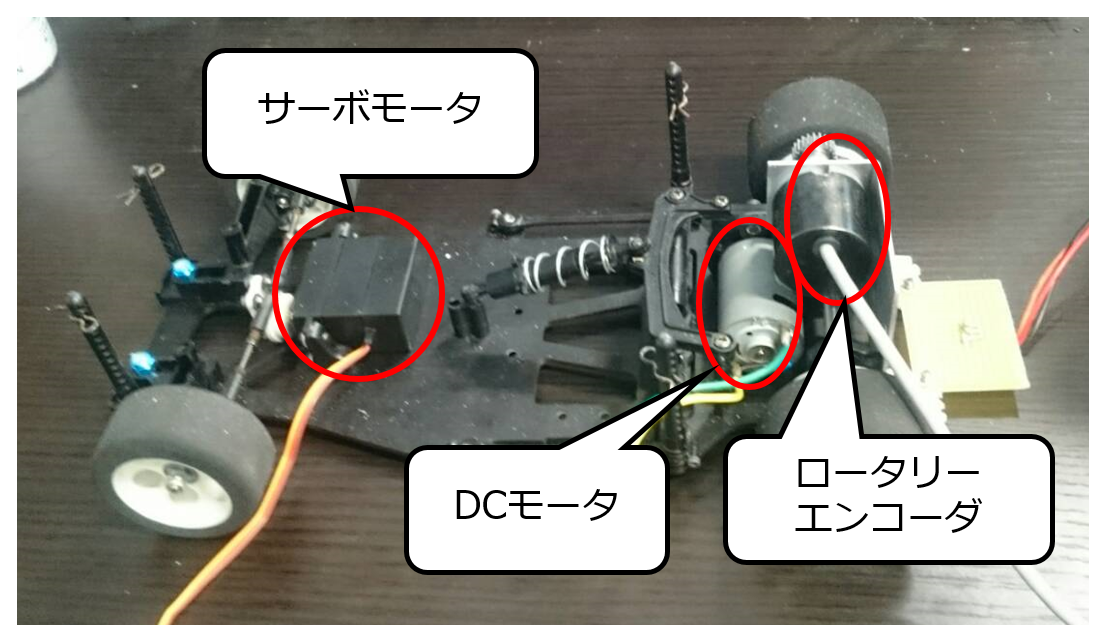
\includegraphics[width=0.5\hsize]{picture/eps/figure1.eps}
  \caption{ロボカーベース部}
  \label{fig::figure1}
\end{figure}

\begin{figure}[htb]
 \centering
  \includegraphics[width=0.5\hsize]{picture/eps/figure2.eps}
  \caption{ロボカー1段目}
  \label{fig::figure2}
\end{figure}

\begin{figure}[htb]
 \centering
  \includegraphics[width=0.5\hsize]{picture/eps/figure3.eps}
  \caption{ロボカー2段目部}
  \label{fig::figure3}
\end{figure}

\begin{figure}[htb]
 \centering
  \includegraphics[width=0.5\hsize]{picture/eps/figure4.eps}
  \caption{ロボカー背面部}
  \label{fig::figure4}
\end{figure}

\newpage
\subsection{ToFセンサ}
今回使用するToFセンサモジュールはデジタル$\mathrm{I^{2}C}$インターフェイスを介して距離を測定しており,2.8$\mathrm{V}$のリニア・レギュレータと,入力電圧2.6$\mathrm{V}$から5.5$\mathrm{V}$までに対応する変圧回路を備えている.また,この距離センサモジュールでは赤外線を使用しており,最大2$\mathrm{m}$まで計測することができて分解能は1$\mathrm{mm}$である.また,以下に仕様を記す\cite{tof_sensor1}.
\begin{itemize}
 \item 動作電圧: 2.6$\mathrm{V}〜5.5\mathrm{V}$
 \item 消費電力: 10$\mathrm{mA}$(通常動作時の平均値)
 \item 検出範囲: 3$\mathrm{cm}〜200\mathrm{cm}$
 \item 重量: 0.5$\mathrm{g}$ (ピンヘッダを除く)
 \item 出力フォーマット$\mathrm{I^{2}C}$: 16ビット読み込み(ミリメートル)
 \item ピンピッチ: 2.54$\mathrm{mm}$ 
\end{itemize}

$\mathrm{5cm}〜\mathrm{70cm}$まで$\mathrm{5cm}$ずつToFセンサで測距を5回ずつ行ってそれらの平均をとってToFセンサの特性実験を行った.横軸に距離の真値,縦軸に距離センサで計測して出力された値とし,距離センサの特性を\refig{tof_graph}のグラフに示す.

\begin{figure}[htb]
  \centering
  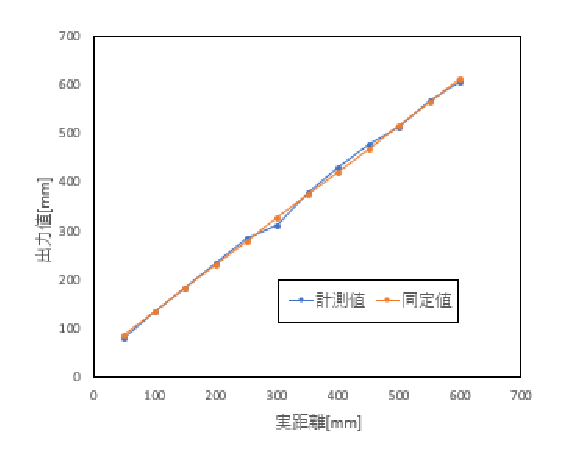
\includegraphics[width=0.5\hsize]{picture/eps/graph.eps}
  \caption{ToFセンサの特性}
  \label{fig::tof_graph}
 \end{figure}

この距離センサを最小二乗法により近似した式は次式となる.なお,$x$は実距離$\mathrm{[mm]}$,$y$は出力値$\mathrm{[mm]}$である.
\begin{equation}
  y = 0.960x + 36.9  \label{eq::1pf}
\end{equation}

\refeq{1pf}より,この式の逆関数を取ることによって計測した距離から実際の距離を導出することができる.$x$を計測して出力された距離$\mathrm{[mm]}$,$d(x)$を実際の距離$\mathrm{[mm]}$とすると次の式となる.

\begin{equation}
  d(x) = 1.04x - 38.4 \label{eq::2pf}
\end{equation}

故に,実際に距離センサでセンシングする際には,\refeq{2pf}によって計測値を実距離へ変換して用いることになる.
また今回は$40\mathrm{mm}$〜$1100\mathrm{mm}$の間でセンシングするため,センシングによって得た値が$40\mathrm{mm}$以下の場合には$40\mathrm{mm}$と,$1100\mathrm{mm}$以上の場合には,$1100\mathrm{mm}$となるような外れ値処理を行った.さらにセンシングで得た値を$0〜1$の間の値で出力するために,センシングで得た値をセンシングの最大値$1100\mathrm{mm}$で割るという正規化処理を施した.

ここで距離センサモジュールの中で使われているI2C(Inter-Integrated Circuit)について説明する.$\mathrm{I^{2}C}$はフィリップス社で開発されたシリアスバスである.$\mathrm{I^{2}C}$の特徴としては,バス・ラインがシリアル・データ・ライン(SDA)とシリアル・クロック・ライン(SCL)の2本のみという簡単な構造の双方向性バスとなっていること,バスの静電容量が400$\mathrm{pF}$以下であれば,1つのバス上にICをいくつでも接続させることが可能であることなどが挙げられる.また,今回のRCRにおいては$\mathrm{I^{2}C}$インターフェイスを介して値を受け渡すのでA/D変換を行わずに測定した距離の値を受け渡すことができるという利点がある\cite{i2c}.

\subsection{ロータリーエンコーダ}
今回使用するロータリーエンコーダ(RE30E-500-213-1)はA相,B相,Z相(ゼロ信号)の3相インクリメンタル型である.
また,今回製作するロボカーは後退しない.つまり,回転方向は考慮しなくても良いため,ロータリーエンコーダの
A相のパルスのみをカウントする.

$k$時点のタイヤの角速度$\omega(k)\unit{rad/s}$は,エンコーダのロータリーエンコーダの一周あたりの
出力パルス数$(500パルス)$,サンプリング周期$(0.005\unit{s})$,ロータリーエンコーダの軸に取り付けた
ピニオンギアとドライブシャフトに取り付けたギア間のギア比$(2.74)$より次式のように算出する.
また,ノイズ対策として算出した角速度を\refeq{lpf}で表されるLow Pass Filterに相当デジタルフィルタ
に通した結果をPublishするようにしている.ただし,$\alpha$は$0〜1$の範囲で定める定数である.\\
      \begin{equation}
      	\omega(k)=\alpha\omega(k)+(1-\alpha)\omega(k-1) \label{eq::lpf}
      \end{equation}

\subsection{フォトリフレクタ}
今回使用するフォトリフレクタ(1RC Reflectance Sensor)は出力がアナログ値でなく2値出力のパルスである.
この出力パルスのパルス幅を計測することによって光の反射率,すなわち床面の色を計測することが出来る.
